\documentclass{article}
\usepackage{graphicx} % Required for inserting images
\usepackage{subcaption}
\usepackage{amssymb}
\usepackage{amsmath} 
\usepackage{ dsfont }
\title{$1-$Dimensional controlled kepler problem}

\begin{document}
\title{$1-$Dimensional controlled kepler problem}


\section{}
About the integration:

From
$$
x'^2 = -2x(x-r_1)(x-r_2)
$$
we find that $v(\tau)$ satisfies 
$$
v'^2 = 4v^3 - g_2 v - g_3,
$$
where  $x(\tau) = -2v(\tau) + \frac{C}{3}$ and
 $$
g_2 = \frac{1}{3}C^2 +1, \qquad  g_3 =- \frac{1}{6}C(1+\frac{2}{9}C^2).
 $$
 Then $v$ is the Weierstrass $\wp$-function and since we have
 $$
\Delta = g_2^3 - 27 g_3^2 > 0
 $$
the fundamental domain is rectangular and
 $$
v(\tau) = \wp(\tau; g_2,g_3) \qquad or \qquad v(\tau) = \wp(\tau+\omega_2; g_2,g_3) 
 $$
where 
\[
\omega_2 = i\int_{-\infty}^{e_3}\frac{dt}{\sqrt{4(e_1-t)(e_2-t)(e_3-t)}}
\]
is the purely imaginary half period and the appropriate choice depends on initial conditions, namely whether the initial value of $v$ lies within $[e_1, \infty)$ or $[e_3, e_2]$.
In our case, the roots of the cubic in $x$ were

 $$
r_1 = \frac{1}{2}(C-\sqrt{C^2+4}) <  0 < r_2 = \frac{1}{2}(C+\sqrt{C^2+4}).
 $$
Thus, the roots in $v$ are
 $$
e_3 = -\frac{C}{12} - \frac{1}{4}\sqrt{C^2+4} \qquad < \qquad e_2 =  \frac{C}{6} \qquad < \qquad e_1 =-\frac{C}{12} + \frac{1}{4}\sqrt{C^2+4}
 $$
where the inequalities hold for every value of $C$.
In order to constraint the motion in the bounded region we need that
 $$
-\frac{C}{12} - \frac{1}{4}\sqrt{C^2+4}  \leq v(0) \leq  \frac{C}{6} 
 $$
or equivalently in $x$
 $$
0 \leq x(0) \leq  r_2 = \frac{1}{2}(C+\sqrt{C^2+4}),
$$
which is always satisfied in our hypothesis. Remark that from
\[
x(\tau) = -2\wp(\tau+\omega_2)+\frac{C}{3},
\]
as the particle approaches the origin in the new time, $x(\tau) \to 0$ we obtain
\[
\tau_c \to \wp^{-1}(\frac{C}{6})-\omega_2 \in \mathds{R}.
\]
From the energy integral one can easily check that
\begin{equation*}
\begin{split}
&|\dot x(t)| \longrightarrow +\infty \qquad \text{as } t \to t_c, \\
& x'(\tau) \longrightarrow 0 \qquad \text{as } \tau  \to \tau_c.
 \end{split}
\end{equation*}
By the relation $d\tau = \frac{1}{x} dt$ we obtain
\begin{equation*}
    \begin{split}
        t = \int_{0}^{\tau} x(\sigma) d\sigma 
         &= -2\int_{0}^{\tau} \wp(\sigma + \omega_2) d\sigma + \frac{C}{3}\tau \\
         &= -2\int_{\omega_2}^{\tau+\omega_2} \wp(s)ds + \frac{C}{3}\tau \\
         &= 2\big(\zeta(\tau + \omega_2) - \zeta(\omega_2)\big) + \frac{C}{3}\tau.
    \end{split}
\end{equation*}

 
 \begin{figure}
\centering
\begin{subfigure}{0.45\textwidth}
  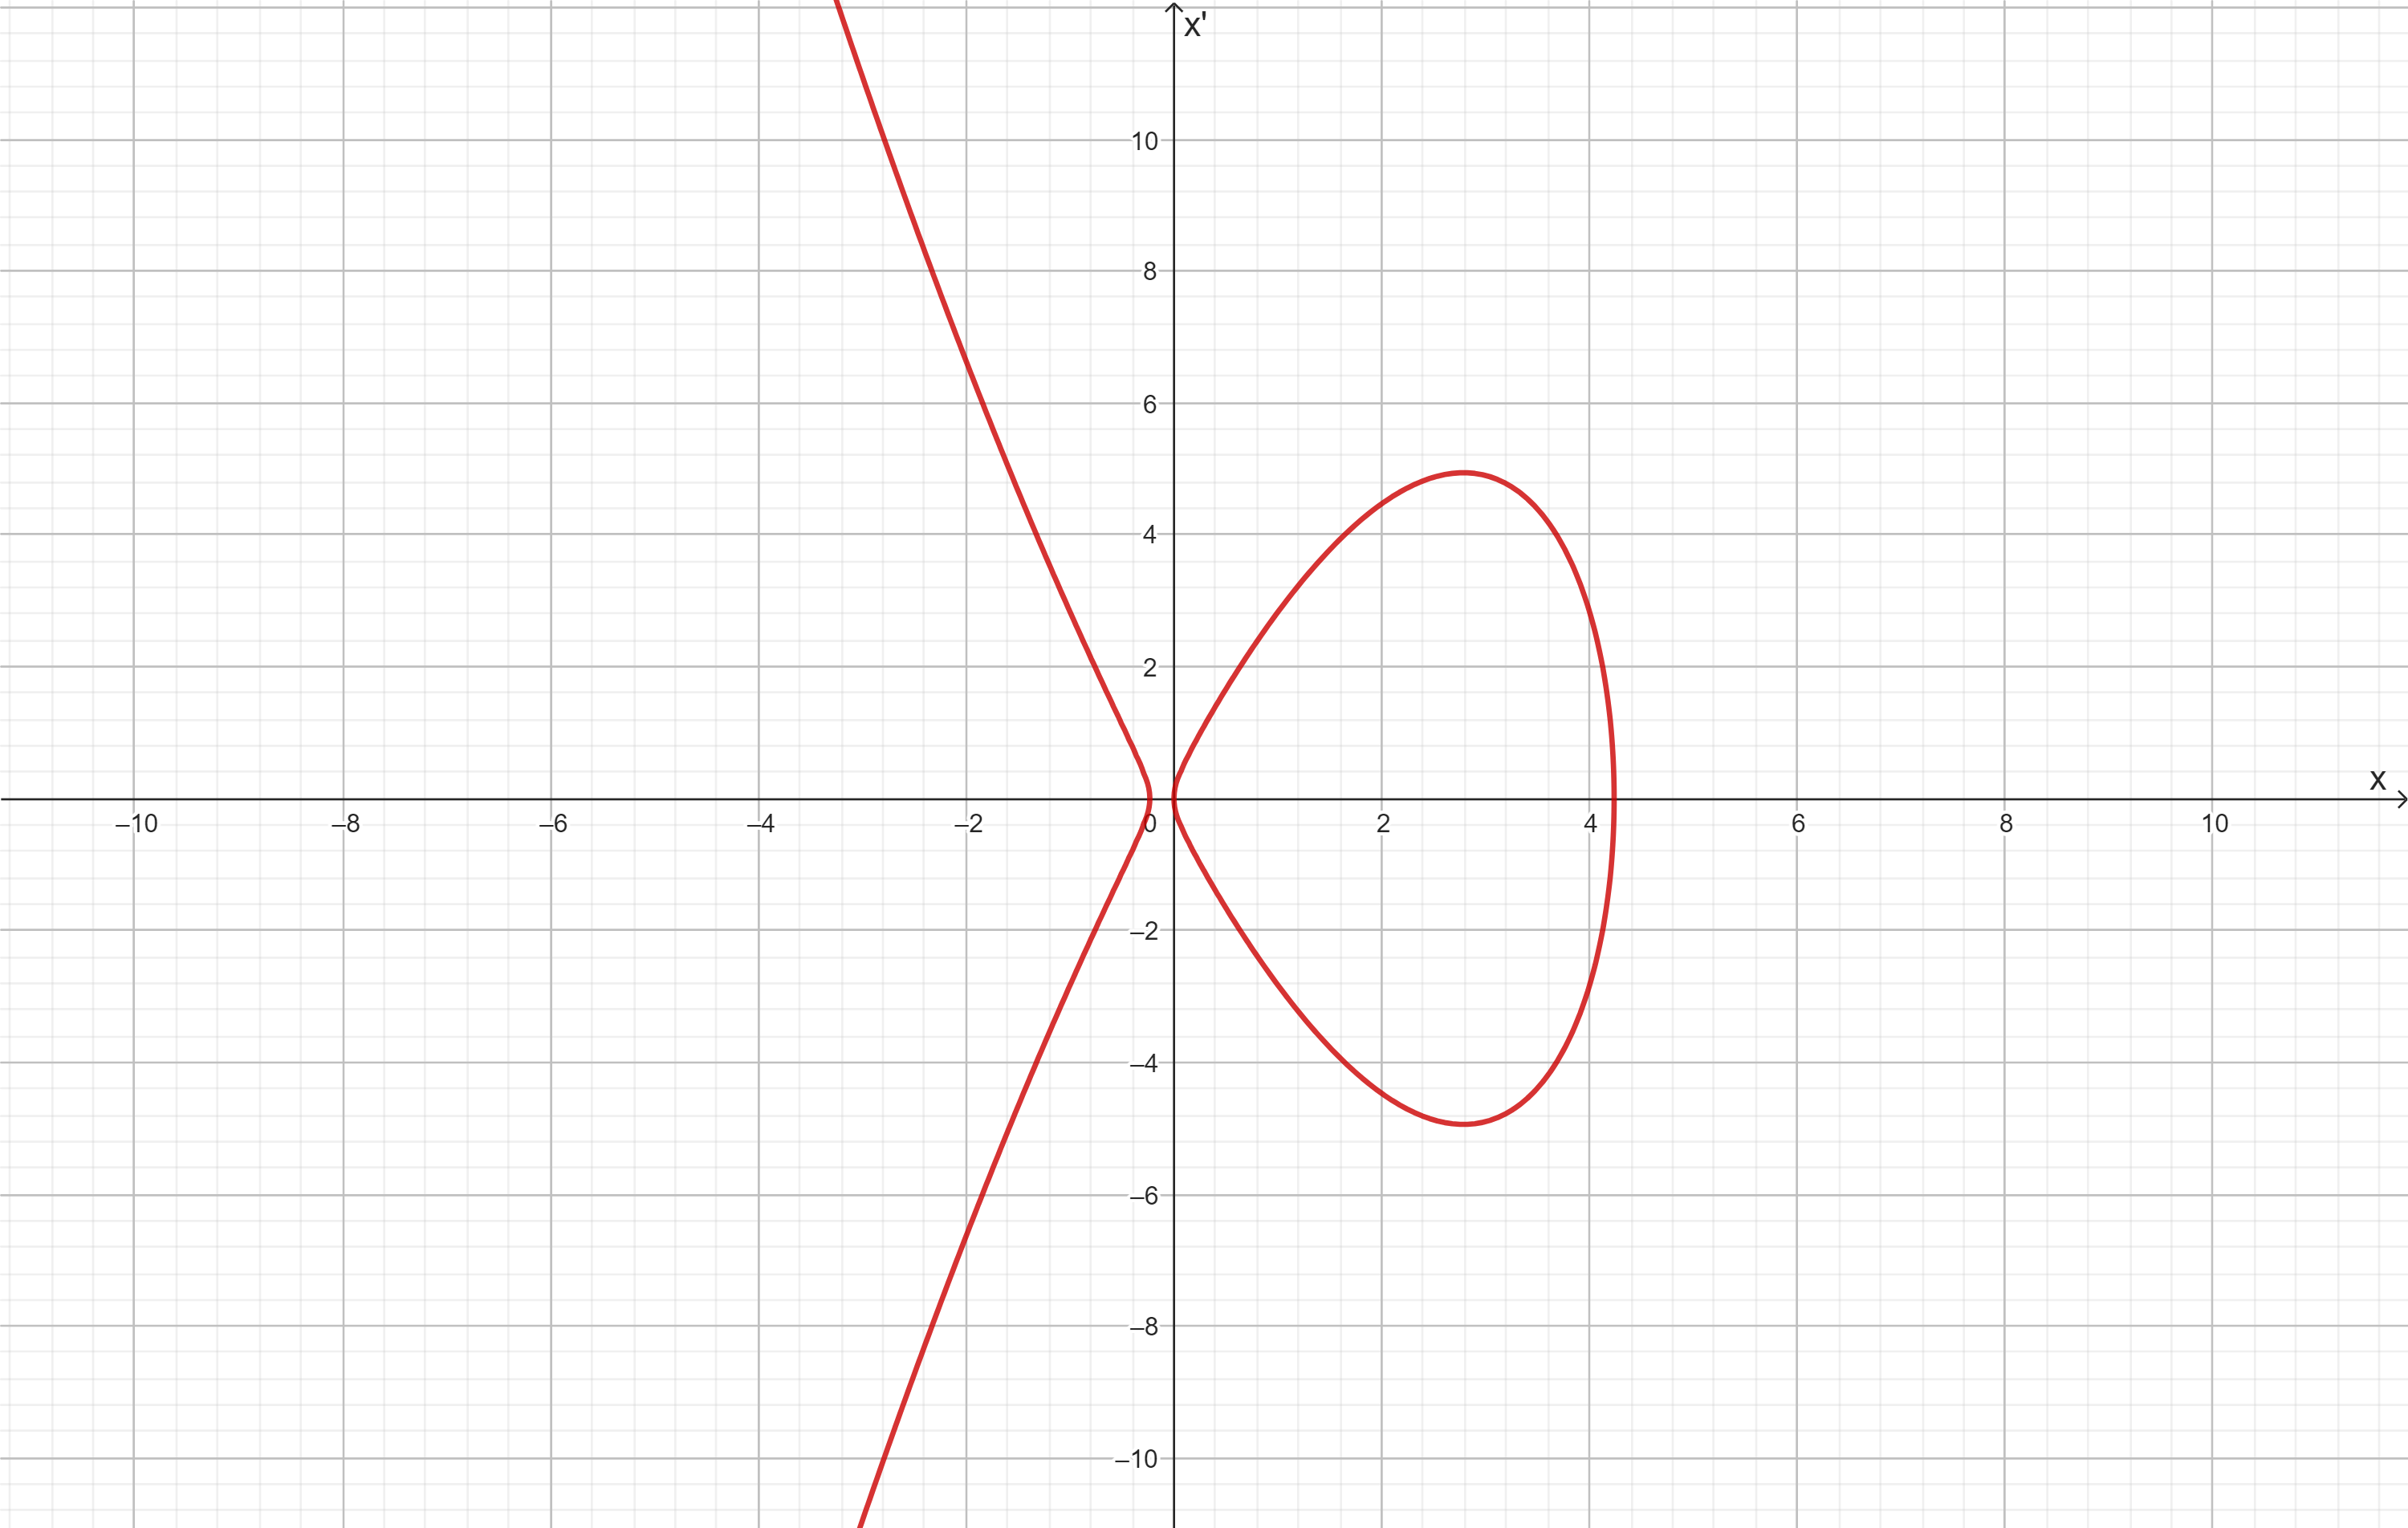
\includegraphics[width=\textwidth]{C=4.png}
  \caption{$C = 4$ }
\end{subfigure}\hfill%\hfill
\begin{subfigure}{0.45\textwidth}
  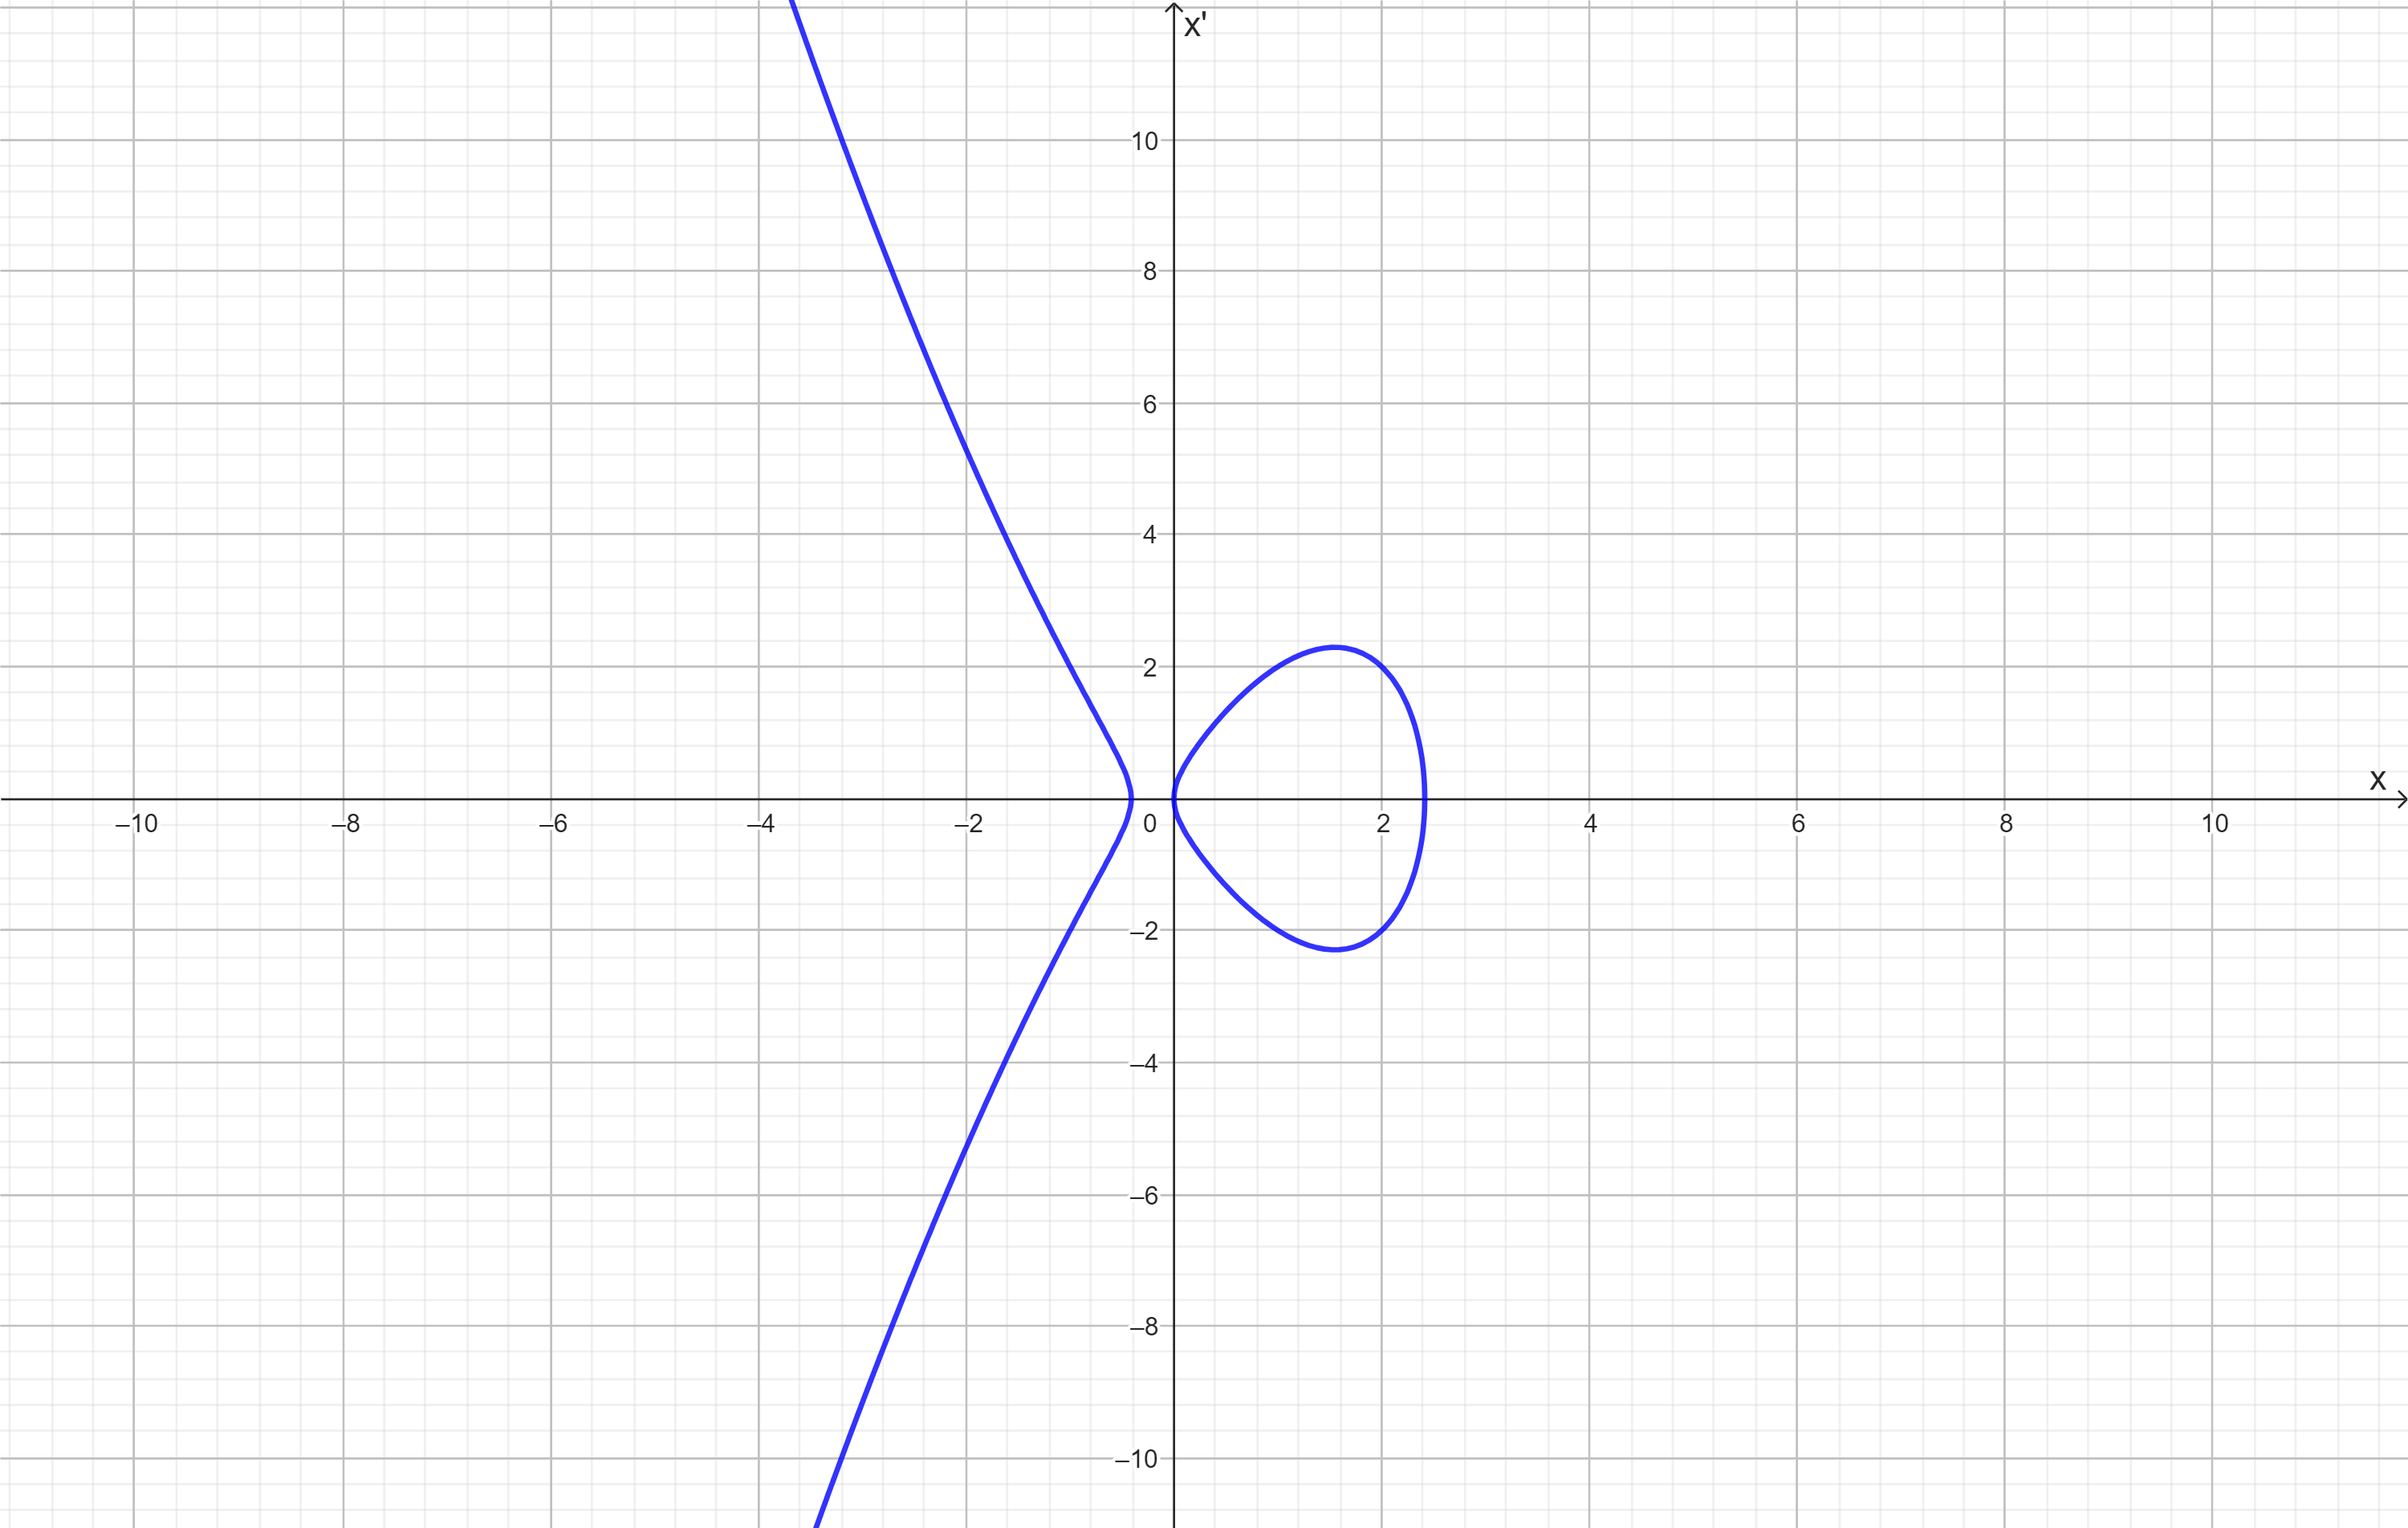
\includegraphics[width=\textwidth]{C=2.png}
  \caption{$C = 2$}
  \end{subfigure}\hfill
  \begin{subfigure}{0.45\textwidth}
  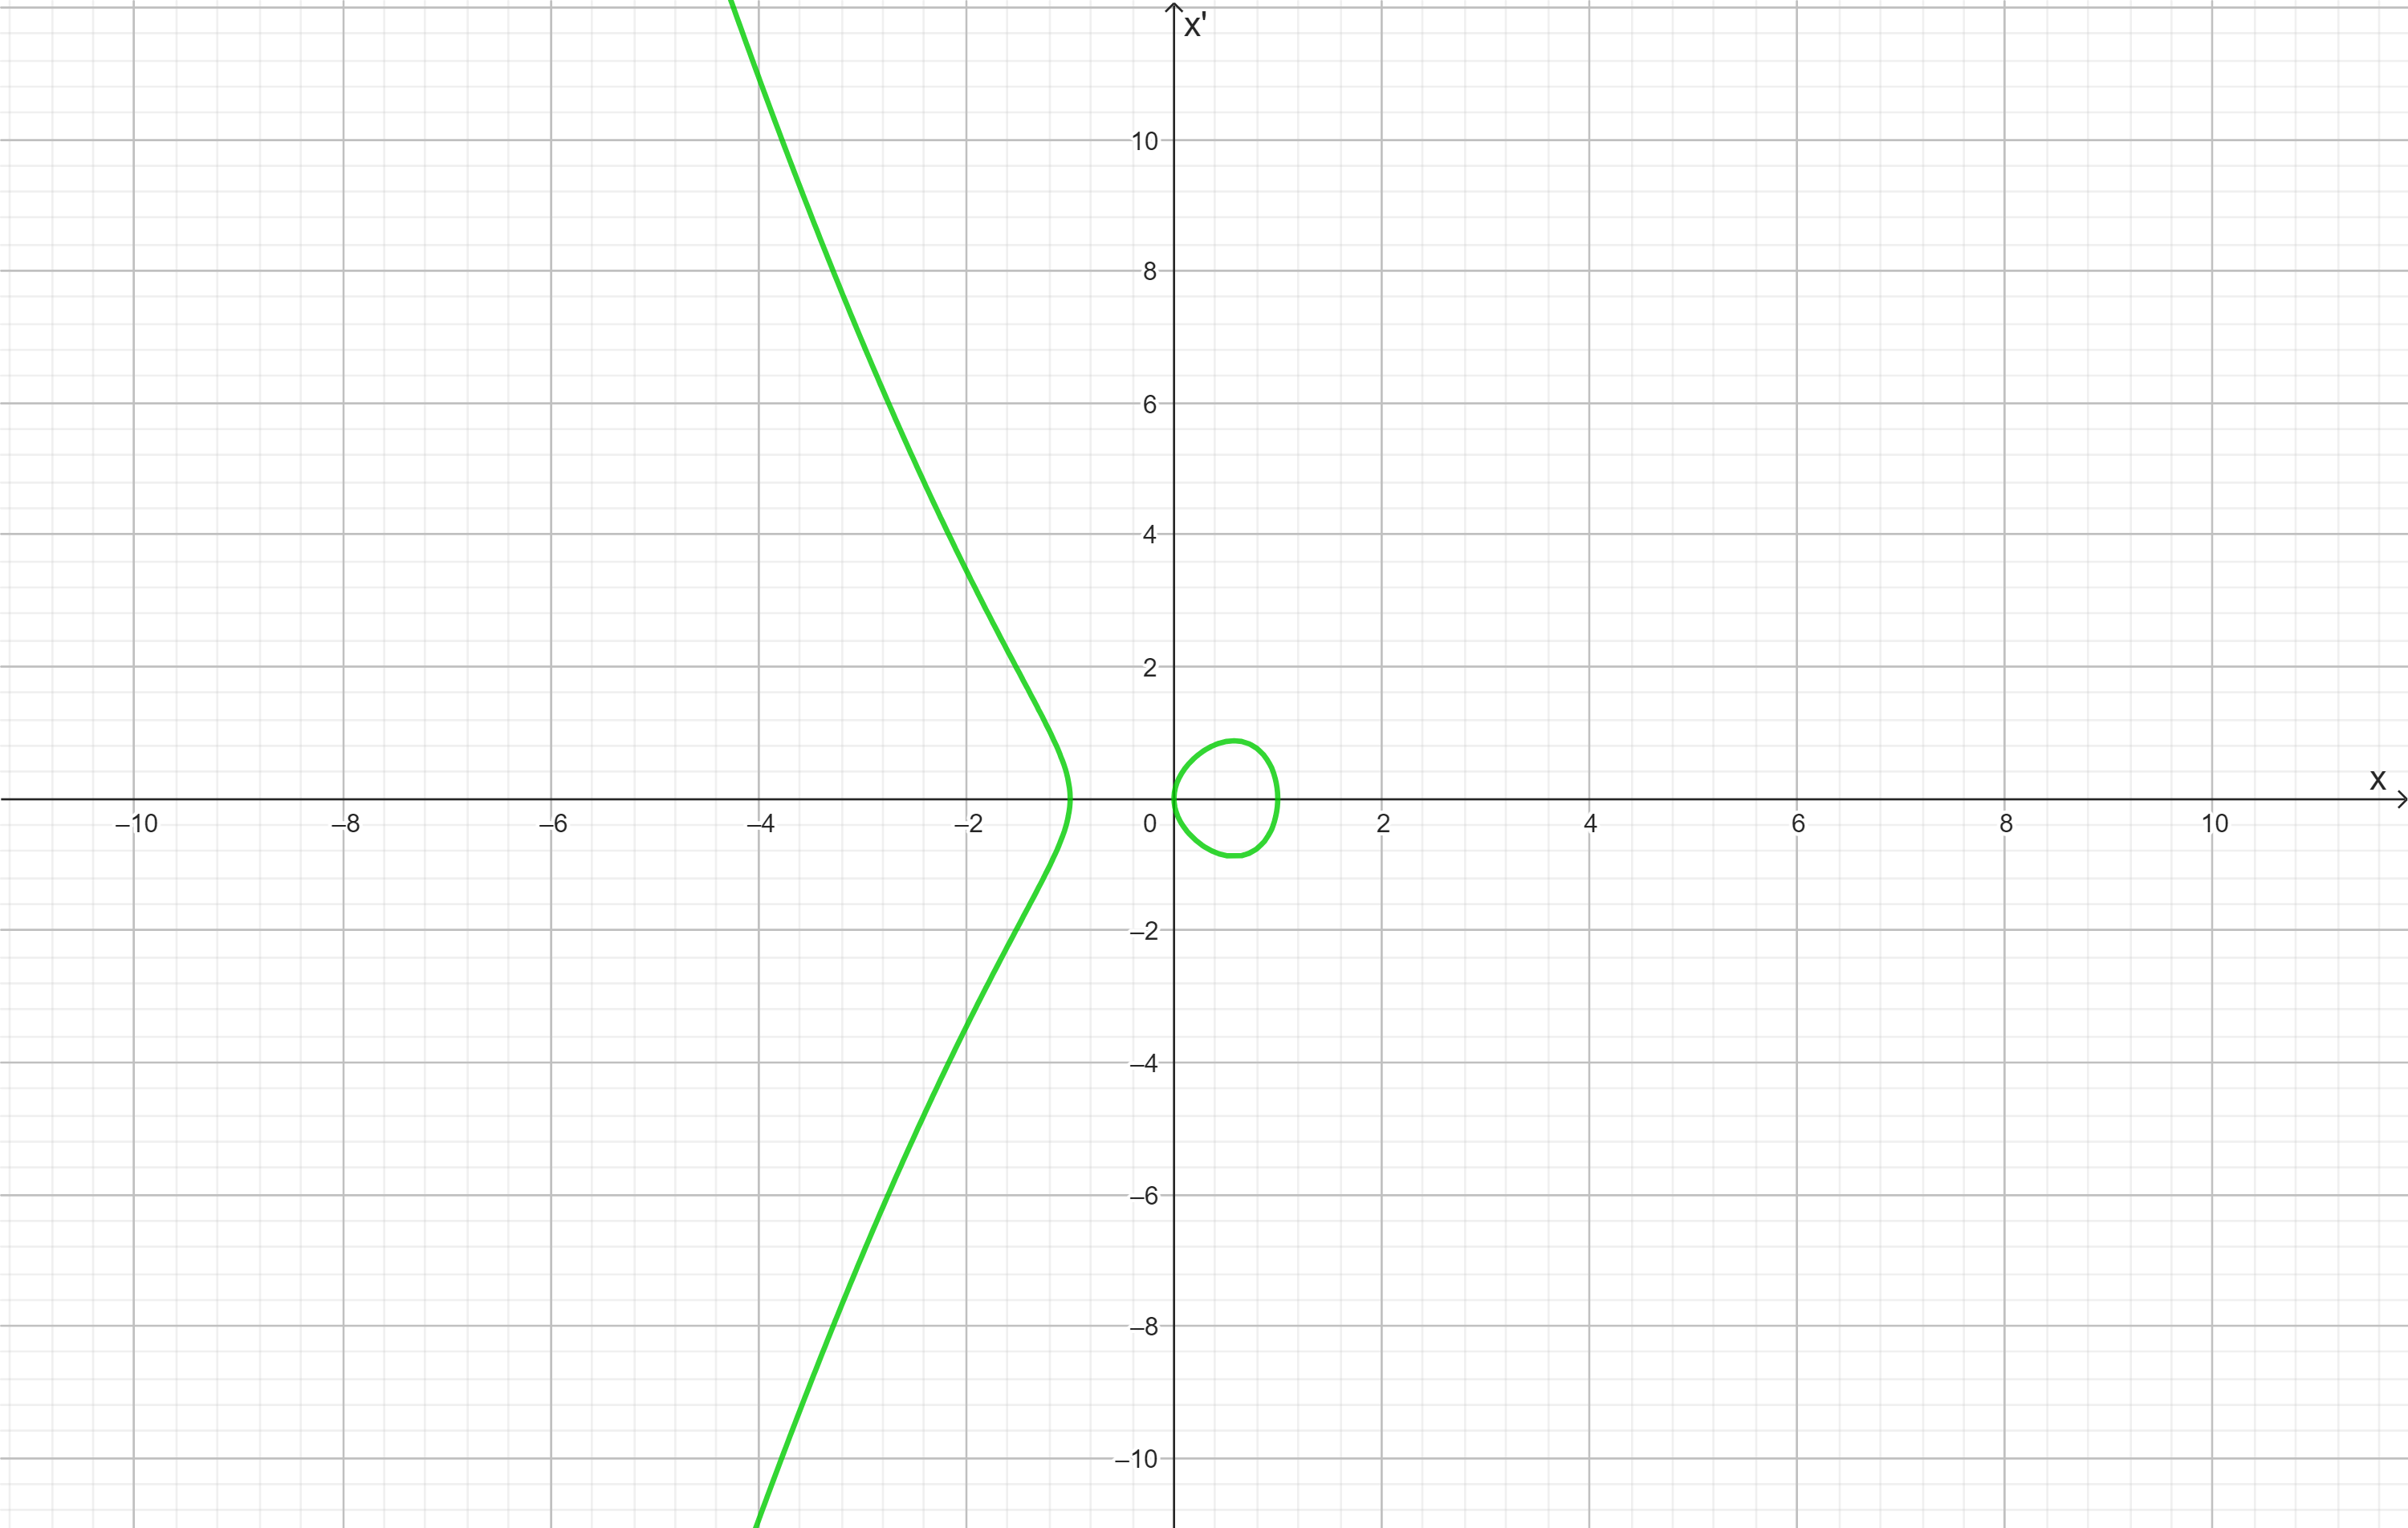
\includegraphics[width=\textwidth]{C=0.png}
  \caption{$C = 0$ }
\end{subfigure}\hfill%
\begin{subfigure}{0.45\textwidth}
  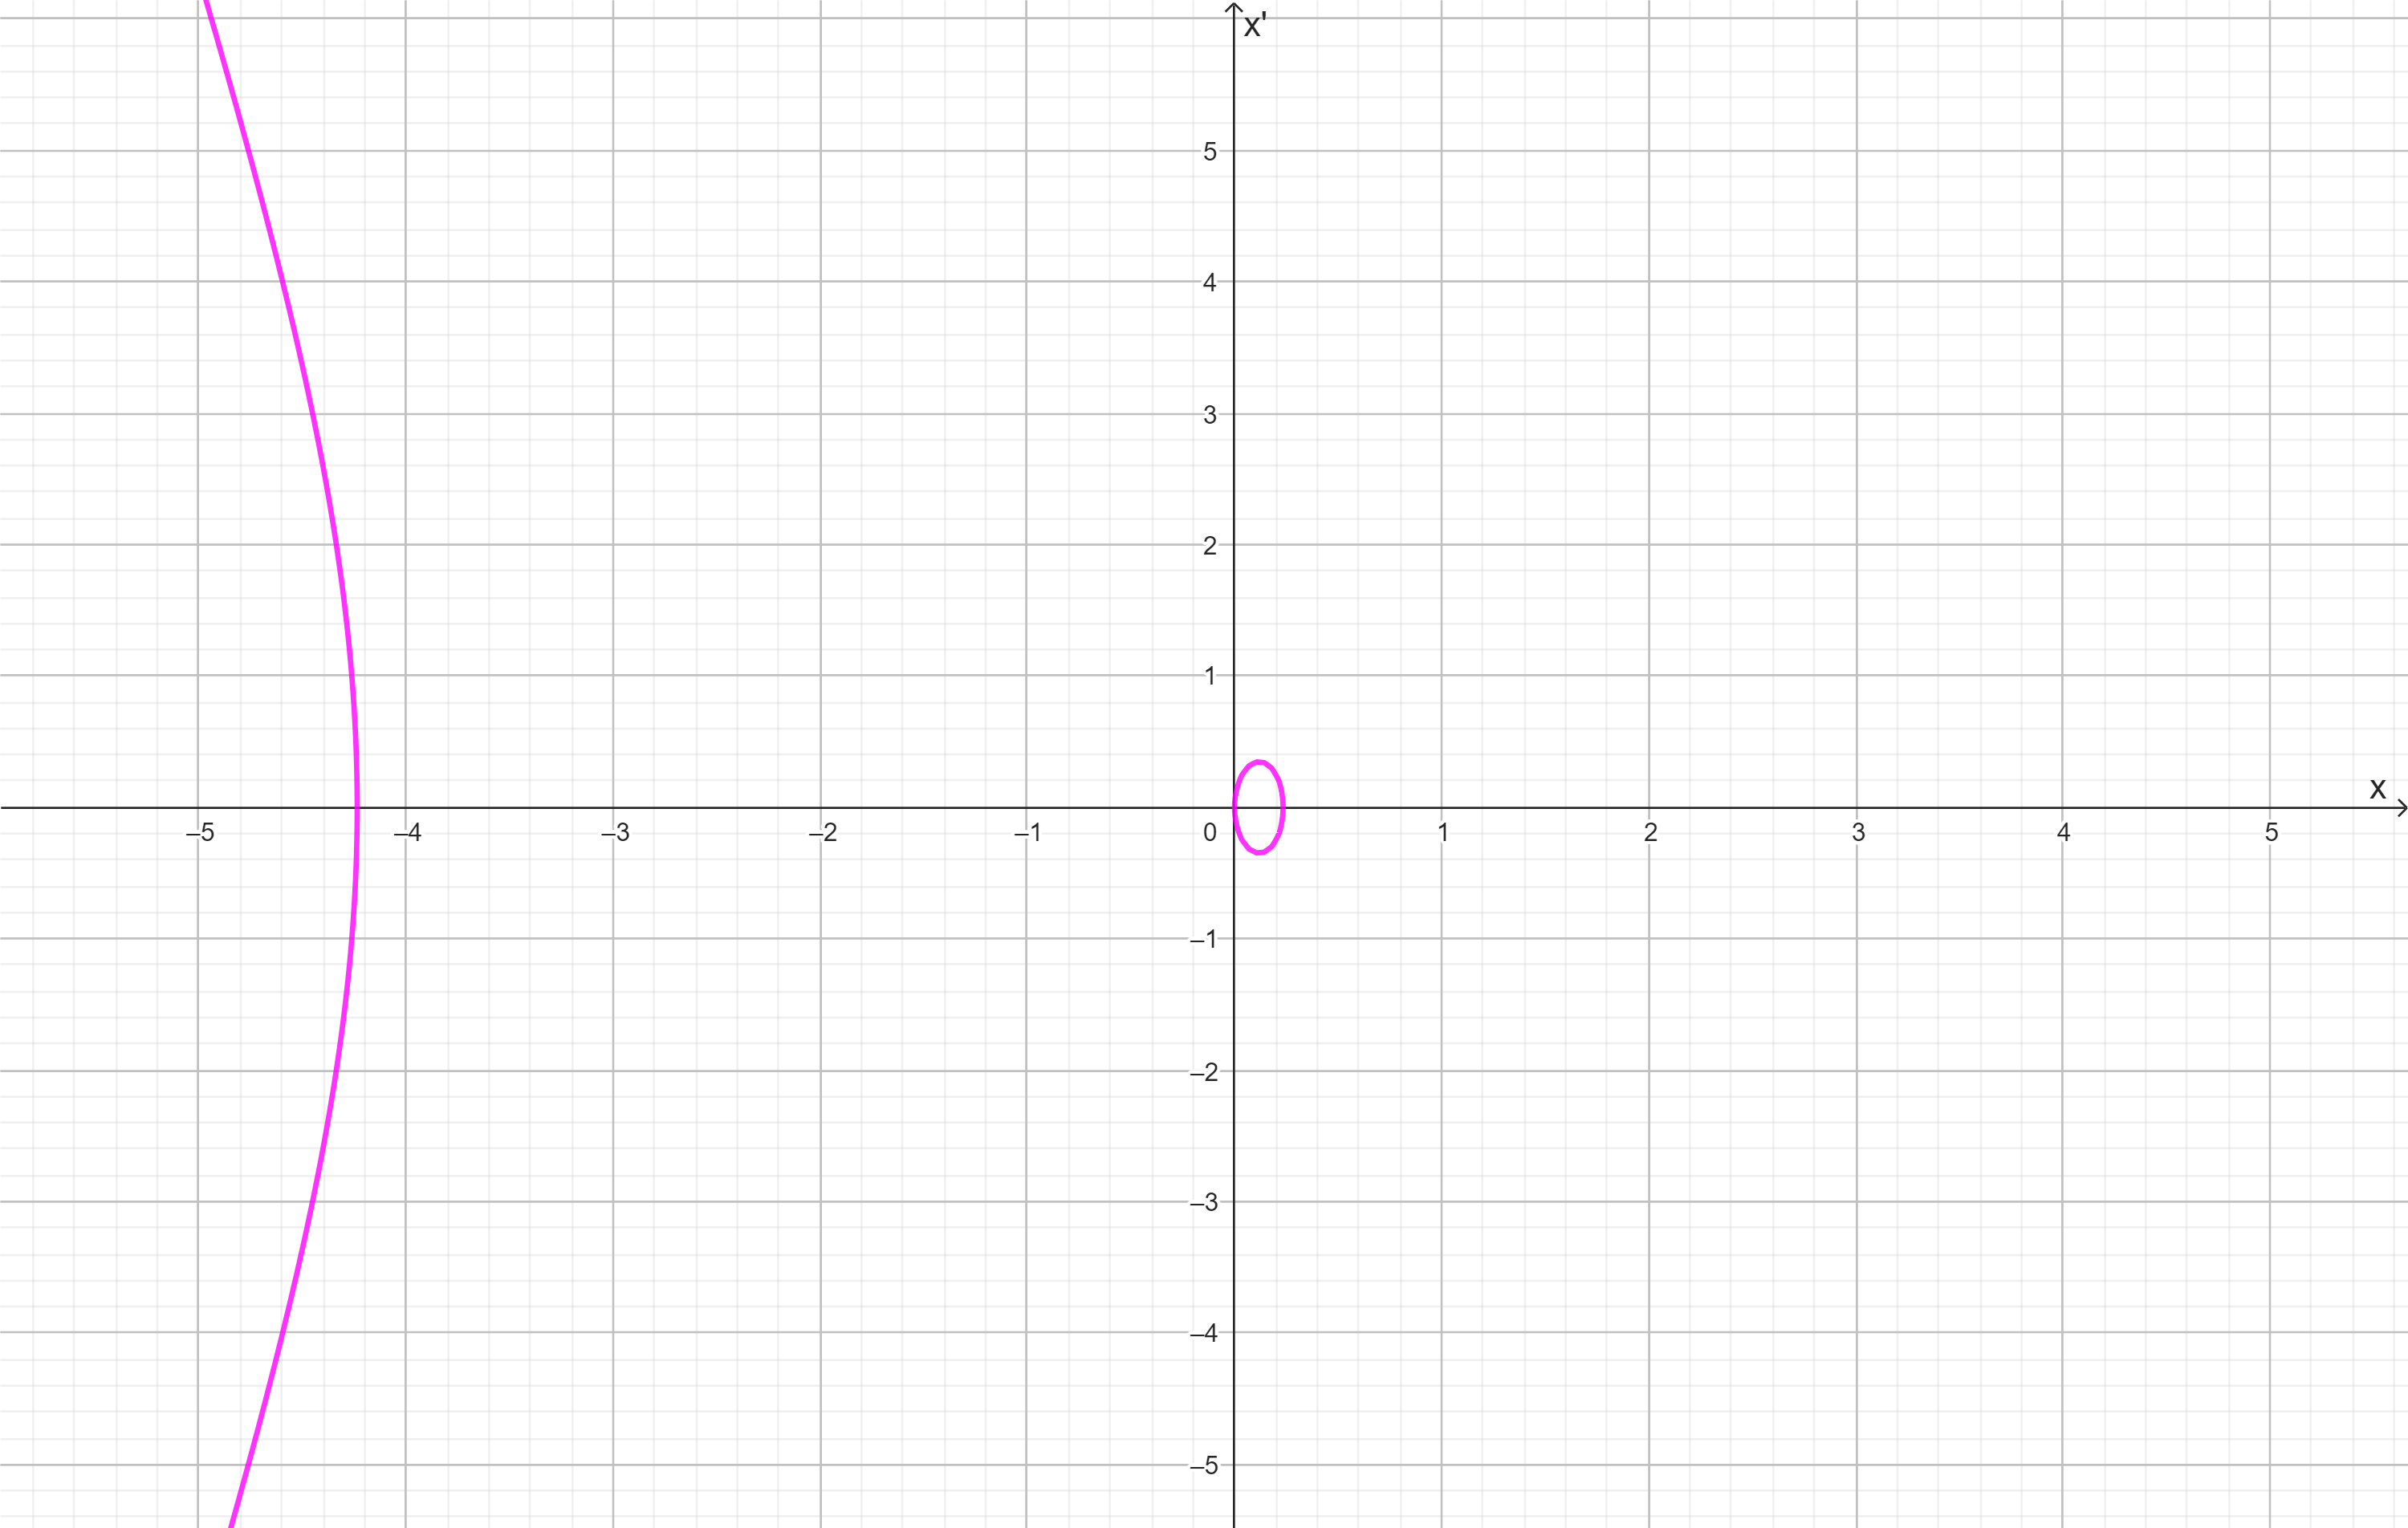
\includegraphics[width=\textwidth]{C=-4.png}
  \caption{$C=-4$}
  \end{subfigure}
\caption{\small{$y^2 = -2x(x-r_1)(x-r_2)$ for different values of $C$.}}
\end{figure}


\newpage

About the \textit{fictitious time} $\tau$: \\
having in mind the equation of motion
\begin{equation}\label{eqmoto}
    \ddot x = -\frac{1}{x^2} - 1
\end{equation}
and the corresponding integral of energy
\begin{equation}\label{energy}
    C = \frac{1}{2}\dot x^2 +x - \frac{1}{x},
\end{equation}
we derive two times the term $x^2$ obtaining
\begin{equation}\label{dxdt}
    \begin{split}
        &\frac{dx^2}{dt} = 2x \dot x, \\
        &\frac{d^2(x^2)}{dt^2} = 2\dot x^2 + 2x \ddot x.
    \end{split}
\end{equation}
From (\ref{energy}) one has
\begin{equation}\label{energy2}
    \dot x^2 = 2(C-x+\frac{1}{x}),
\end{equation}
which implies that $\dot x \sim x^{-\frac{1}{2}}$ as $t \to t_c$. From (\ref{eqmoto}), (\ref{dxdt}) and (\ref{energy2}) it is found
\begin{equation*}
\begin{split}
    \frac{d^2(x^2)}{dt^2} &= 4(C-x+\frac{1}{x}) +2x(-\frac{1}{x^2} - 1) \\
    & = 4C - 6x + \frac{2}{x}.
    \end{split}
\end{equation*}
The function $4C-6x$ is well defined and finite at collision, hence by integrating the last expression one has
\begin{equation}
    2\int_{t_0}^{t} \frac{1}{x}dt = \int_{t_0}^{t} \frac{d^2(x^2)}{dt^2}dt - \int_{t_0}^{t} (4C-6x)dt < \infty \text{ as } t\to t_c,
\end{equation}
since  $\frac{dx^2}{dt} = 2x \dot x \sim x^{\frac{1}{2}} \to 0$ as $t \to t_c$. Then $\tau$ defined by the differential relation $d\tau = \frac{1}{x}dt$ is a monotone function well-defined at collision.
\end{document}
